\documentclass[crop,tikz]{standalone}
\usepackage{tikz}
\usepackage{xcolor}
\usetikzlibrary{backgrounds,calc,shapes,arrows,decorations.pathreplacing,decorations.markings,patterns,positioning,3d,fit,shapes.geometric,fadings}

% Define colors
\definecolor{nodecolor1}{RGB}{31, 119, 180}
\definecolor{nodecolor2}{RGB}{255, 127, 14}
\definecolor{nodecolor3}{RGB}{44, 160, 44}
\definecolor{nodecolor4}{RGB}{214, 39, 40}
\definecolor{nodecolor5}{RGB}{148, 103, 189}
\definecolor{edgecolor1}{RGB}{150, 150, 150}
\definecolor{edgecolor2}{RGB}{100, 100, 100}
\definecolor{background}{RGB}{252, 252, 252}

\begin{document}
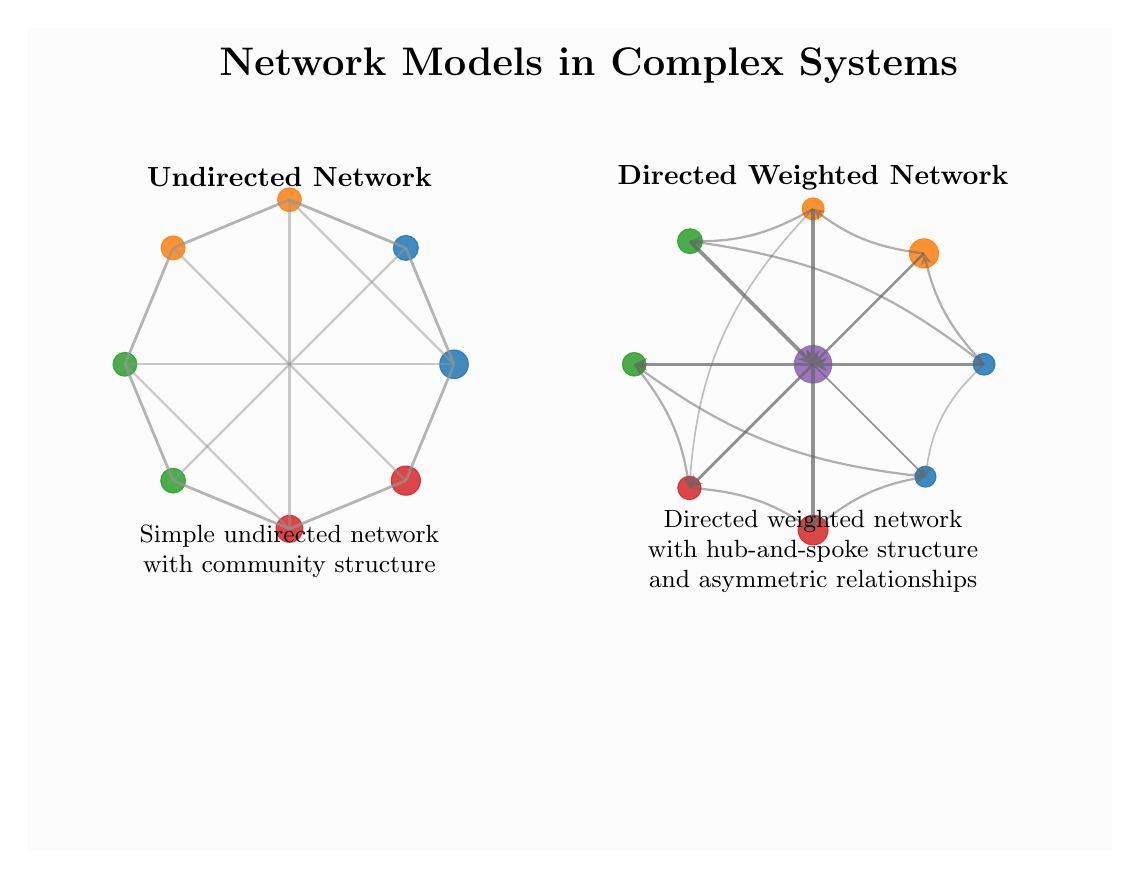
\begin{tikzpicture}[scale=0.95]
  % Set background color
  \fill[background] (-0.5,-0.5) rectangle (14,10.5);

  % Title
  \node[font=\Large\bfseries] at (7,10) {Network Models in Complex Systems};

  % Basic undirected graph
  \node[font=\bfseries] at (3,8.5) {Undirected Network};

  % Create nodes with different sizes and colors
  \def\radius{2.2}
  \def\nodenum{8}

  % Calculate positions of nodes in a circle
  \foreach \i in {1,...,\nodenum} {
    \pgfmathsetmacro{\angle}{(\i-1)*360/\nodenum}
    \pgfmathsetmacro{\x}{3 + \radius*cos(\angle)}
    \pgfmathsetmacro{\y}{6 + \radius*sin(\angle)}
    \pgfmathsetmacro{\size}{0.15 + 0.05*rnd}

    % Choose node color based on index
    \ifnum\i<3
      \def\nodecolor{nodecolor1}
    \else\ifnum\i<5
      \def\nodecolor{nodecolor2}
    \else\ifnum\i<7
      \def\nodecolor{nodecolor3}
    \else
      \def\nodecolor{nodecolor4}
    \fi\fi\fi

    % Draw the node
    \coordinate (N\i) at (\x,\y);
    \filldraw[\nodecolor, opacity=0.85] (N\i) circle (\size);
  }

  % Create edges with varying thickness
  \draw[edgecolor1, opacity=0.7, line width=1pt] (N1) -- (N2);
  \draw[edgecolor1, opacity=0.7, line width=1pt] (N2) -- (N3);
  \draw[edgecolor1, opacity=0.7, line width=1pt] (N3) -- (N4);
  \draw[edgecolor1, opacity=0.7, line width=1pt] (N4) -- (N5);
  \draw[edgecolor1, opacity=0.7, line width=1pt] (N5) -- (N6);
  \draw[edgecolor1, opacity=0.7, line width=1pt] (N6) -- (N7);
  \draw[edgecolor1, opacity=0.7, line width=1pt] (N7) -- (N8);
  \draw[edgecolor1, opacity=0.7, line width=1pt] (N8) -- (N1);

  % Add some cross-connections
  \draw[edgecolor1, opacity=0.5, line width=0.8pt] (N1) -- (N5);
  \draw[edgecolor1, opacity=0.5, line width=0.8pt] (N2) -- (N6);
  \draw[edgecolor1, opacity=0.5, line width=0.8pt] (N3) -- (N7);
  \draw[edgecolor1, opacity=0.5, line width=0.8pt] (N4) -- (N8);
  \draw[edgecolor1, opacity=0.5, line width=0.8pt] (N1) -- (N3);
  \draw[edgecolor1, opacity=0.5, line width=0.8pt] (N5) -- (N7);

  % Annotations
  \node[align=center, font=\small] at (3,3.5) {Simple undirected network\\with community structure};

  % Directed graph with weights
  \node[font=\bfseries] at (10,8.5) {Directed Weighted Network};

  % Create a more complex directed network
  % Central hub
  \coordinate (H) at (10,6);
  \filldraw[nodecolor5, opacity=0.9] (H) circle (0.25);

  % Surrounding nodes
  \foreach \i in {1,...,8} {
    \pgfmathsetmacro{\angle}{(\i-1)*360/8}
    \pgfmathsetmacro{\r}{2.0+0.4*rnd}
    \pgfmathsetmacro{\x}{10 + \r*cos(\angle)}
    \pgfmathsetmacro{\y}{6 + \r*sin(\angle)}
    \pgfmathsetmacro{\size}{0.12 + 0.08*rnd}

    % Choose node color based on angle quadrant
    \pgfmathsetmacro{\quadrant}{int(mod(floor((\angle+45)/90),4))}
    \ifnum\quadrant=0
      \def\nodecolor{nodecolor1}
    \else\ifnum\quadrant=1
      \def\nodecolor{nodecolor2}
    \else\ifnum\quadrant=2
      \def\nodecolor{nodecolor3}
    \else
      \def\nodecolor{nodecolor4}
    \fi\fi\fi

    % Draw the node
    \coordinate (D\i) at (\x,\y);
    \filldraw[\nodecolor, opacity=0.85] (D\i) circle (\size);

    % Draw directed edges with varying thickness
    \pgfmathsetmacro{\thickness}{0.4 + 1.0*rnd}

    % Inward edges from outer nodes to center
    \ifnum\i<5
      \draw[->, >=stealth, edgecolor2, opacity=0.7, line width=\thickness pt] (D\i) -- (H);
    \else
      % Outward edges from center to outer nodes
      \draw[->, >=stealth, edgecolor2, opacity=0.7, line width=\thickness pt] (H) -- (D\i);
    \fi
  }

  % Add connections between outer nodes
  \draw[->, >=stealth, edgecolor2, opacity=0.5, line width=0.8pt] (D1) to[bend left=15] (D2);
  \draw[->, >=stealth, edgecolor2, opacity=0.5, line width=0.8pt] (D2) to[bend left=15] (D3);
  \draw[->, >=stealth, edgecolor2, opacity=0.5, line width=0.8pt] (D3) to[bend left=15] (D4);
  \draw[->, >=stealth, edgecolor2, opacity=0.5, line width=0.8pt] (D4) to[bend left=15] (D1);

  \draw[->, >=stealth, edgecolor2, opacity=0.5, line width=0.8pt] (D5) to[bend left=15] (D6);
  \draw[->, >=stealth, edgecolor2, opacity=0.5, line width=0.8pt] (D6) to[bend left=15] (D7);
  \draw[->, >=stealth, edgecolor2, opacity=0.5, line width=0.8pt] (D7) to[bend left=15] (D8);
  \draw[->, >=stealth, edgecolor2, opacity=0.5, line width=0.8pt] (D8) to[bend left=15] (D5);

  % Add some random cross connections
  \draw[->, >=stealth, edgecolor2, opacity=0.4, line width=0.6pt] (D1) to[bend right=20] (D8);
  \draw[->, >=stealth, edgecolor2, opacity=0.4, line width=0.6pt] (D3) to[bend right=20] (D6);

  % Annotations
  \node[align=center, font=\small] at (10,3.5) {Directed weighted network\\with hub-and-spoke structure\\and asymmetric relationships};

\end{tikzpicture}
\end{document}